<%# some convenience definitions %>
<%# wiki = @wiki %>
<% full = wiki.filter.clone; full.include_all_namespaces %>
<% wiki.filter.namespace=0 %>
<% users = @wiki.users %>
<% pages = @wiki.pages %>
<% revisions = @wiki.revisions %>
\documentclass{scrartcl}

\usepackage[T1]{fontenc}
\usepackage{booktabs}
\usepackage{graphicx}
\usepackage{tabularx}

\title{Mediawiki Report -- <%= wiki.to_s %>
}
\author{mediawikiparser (<\texttt{klaus.stein@uni-bamberg.de}>)}


\begin{document}
\maketitle


\section{Statistics} % (fold)
\label{sec:statistics}

We have <%=@wiki.pages(full).length%> pages with 
<%=@wiki.revisions(full).length%>  revisions from <%=users.length%> 
users (<%=pages.length%> pages with <%=revisions.length%> revisions in 
Namespace 0).

\subsection{Wiki Statistics} % (fold)
\label{sub:wiki_statistics}

\begin{tabular}{>{\bfseries}lrrrrr}\toprule
  &\textbf{avg} &\textbf{stddev} &\textbf{med} &\textbf{min}
  &\textbf{max}\\
\midrule
<%= 
wiki.global_userstats.collect { |a|
  a.collect { |v| 
    if v.kind_of?(String)
      v
    elsif v.integer? 
      '%5i' % v
    elsif v.nan?
      '---'
    else
      '%7.2f' % v
    end
  }.join('&')
}.join('\\\\')
%>      
\\\bottomrule
\end{tabular}

% subsection wiki_statistics (end)

\subsection{User Statistics} % (fold)
\label{sub:user_statistics}

\begin{tabular}{>{\bfseries}llrrrrr}\toprule
\textbf{User} & & \textbf{\#edits} & \textbf{\#pages} &
\textbf{edits/page} & \textbf{\#self edits} & \textbf{\#foreign
  edits}\\
\midrule
<%= 
wiki.userstats.sort_by { |u,| u.name }.collect { |u,values| 
  ([u.name, u.node_id] + values[0..4].collect { |v|
     if v.kind_of?(String)
       v
     elsif v.integer? 
       '%5i' % v
     elsif v.nan?
       '---'
     else
       '%7.2f' % v
     end
   }).join('&')
}.join('\\\\')
%>
\\\bottomrule
\end{tabular}

% subsection user_statistics (end)

% section statistics (end)


%%% Cummulative Distribution Functions: Lorenz, Gini, Pareto %%%

\section{Cummulative Distribution Functions} % (fold)
\label{sec:cummulative_distribution_functions}

% Authors vs. Revisions
<%
ur = users.collect { |u| u.revisions.length }
ur.gp_plot_lorenz(:title => "Lorenz Curve", :xlabel => "authors",
 :ylabel => "revisions", :png => 'cdfar.png', :size => '480,480')
%>
\begin{center}
  \includegraphics[width=\textwidth]{cdfar.png}
\end{center}

% Authors vs. Pages
<%
up = users.collect { |u| u.pages.length }
up.gp_plot_lorenz(:title => "Lorenz Curve", :xlabel => "authors", :ylabel => "pages", :png=>'cdfap.png', :size => '480,480')
%>
\begin{center}
  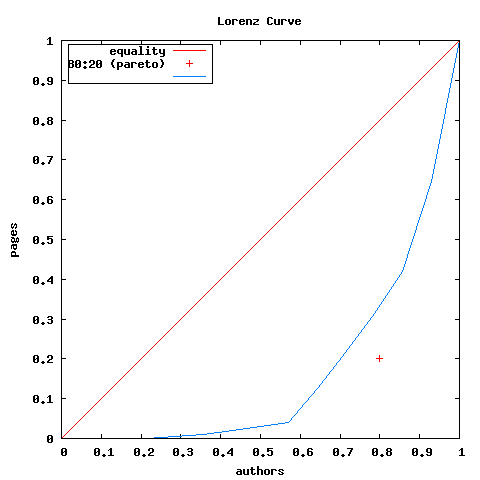
\includegraphics[width=\textwidth]{cdfap.png}
\end{center}

% Revisions vs. Pages
<%
pr = pages.collect { |p| p.revisions.length }
pr.gp_plot_lorenz(:title => "Lorenz Curve", :xlabel => "pages", :ylabel => "revisions", :svg=>'cdfpr.svg')
pr.gp_plot_lorenz(:title => "Lorenz Curve", :xlabel => "pages", :ylabel => "revisions", :png=>'cdfpr.png', :size => '480,480')
%>
\begin{center}
  \includegraphics[width=\textwidth]{cdfpr.png}
\end{center}

% section cummulative_distribution_functions (end)


%%% Set Filter and Time Raster %%%
<%
filter = wiki.filter.clone # clone filter
raster = wiki.timeraster(:zero => :month, :step => :month) # set time raster to monthly spells
%>

\section{Revision History} % (fold)
\label{sec:revision_history}

% Cummulative Revisions per Month (CRPM)
<% 
crpm = raster[1..-2].collect { |e| filter.endtime = e 
	[ e, wiki.revisions(filter).length ]
	}
Gnuplot.new do |gp|
	gp.set('xdata', 'time')
	gp.set('timefmt', '%Y-%m-%d', true)
	gp.set('format x', '%b %y', true)
	gp.add(crpm, :timefmt => '%Y-%m-%d', 
		:with => 'linespoints', 
		:title => 'revisions')
	gp.set('nokey')
	gp.set('xtics rotate')
	gp.set('title "Cummulative Revisions per Month"')
	gp.set('xlabel "month"')
	gp.set('ylabel "cummulative number of revisions"')
	gp.plot(:svg => 'crpm.svg')
	gp.plot(:png => 'crpm.png', :size => '640,480')
end
%>
\begin{center}
  \includegraphics[width=\textwidth]{crpm.png}
\end{center}

% Revisions per Month (RPM)
<% 
rpm = raster[1..-2].enum_cons(2).collect { |s,e| 
	filter.revision_timespan = (s..e)
	[ e, wiki.revisions(filter).length ]
	}
Gnuplot.new do |gp|
	gp.set('xdata', 'time')
	gp.set('timefmt', '%Y-%m-%d', true)
	gp.set('format x', '%b %y', true)
	gp.add(rpm, :timefmt => '%Y-%m-%d',
		:with => 'lines', 
		:title => 'revisions' )
	gp.set('xtics rotate')
	gp.set('title "Revisions per Month"')
	gp.set('xlabel "month"')
	gp.set('ylabel "number of revisions"')
	gp.fit(:title => 'trend')
	gp.plot(:svg => 'rpm.svg')
	gp.plot(:png => 'rpm.png', :size => '640,480')
end
%>
\begin{center}
  \includegraphics[width=\textwidth]{rpm.png}
\end{center}

% section revision_history (end)

\section{Author Participation} % (fold)
\label{sec:author_participation}

% Author Participation
<%
# events
events = wiki.users.collect{ |u| 
	[ u.time_of_first_event, u.time_of_last_event ] 
    }.select { |f,l| f && l }
# authors
authors = raster.enum_cons(2).collect { |s,e|
	filter.revision_timespan = (s..e)
	[ e,
    	wiki.coauthorgraph(filter).remove_lonely_nodes.nodes.length /
        events.reject { |f,l| (f > e) || (l < s) }.length.to_f ]
	}[1..-2]
# Gnuplot
Gnuplot.new do |gp|
	gp.set('xdata', 'time')
	gp.set('timefmt', '%Y-%m-%d', true)
	gp.set('format x', '%b %y', true)
	gp.add(authors, :timefmt => '%Y-%m-%d',
		:with => 'lines',
		:title => 'authors')
	gp.set('nokey')
	gp.set('xtics rotate')
	gp.set('title "Author Participation"')
	gp.set('xlabel "month"')
	gp.set('ylabel "percentage of authors"')
	gp.fit(:title => 'trend')
	gp.plot(:svg => 'rap.svg')
	gp.plot(:png => 'rap.png', :size => '640,480')
end
%>
\begin{center}
  \includegraphics[width=\textwidth]{rap.png}
\end{center}

% section author_participation (end)

\section{Network Visualization} % (fold)
\label{sec:network_visualization}

% Co-Authorship Network
<%
wiki.coauthorgraph.r_plot(:filename => "coauthorgraph.png")
%>
\begin{figure}
	\centering
	\includegraphics[width=\textwidth]{coauthorgraph.png}
	\caption{Co-Authorship Network}
	\label{fig:co-authorship_network}
\end{figure}

% Document Network
<%
wiki.pagegraph.r_plot(:filename => "pagegraph.png")
%>

\begin{figure}
	\centering
	\includegraphics[width=\textwidth]{pagegraph.png}
	\caption{Document Network}
	\label{fig:document_network}
\end{figure}

Figure~\ref{fig:document_network} displays the wiki's document network. Nodes are wiki pages, edges are hyperlinks from one to another page. 

% wiki.pagegraph.degrees.collect {|k,v| [ k, v[1]/1 ]}.sort_by { |k,v| -v }.collect { |k,v| [ k.title, v] }[0..4]



% section network_visualization (end)



\end{document}
